\chapter{Elementos Pós Textuais}
\section{Bibliografia}

Para criar um bibliografia, vá na pasta ``bibliografia'' dentro da pasta ``elementosPosTextuais'' e edite o arquivo. Existem vários tipos de bibliografias que se podem utilizar, como por exemplo:

\begin{table}[htb]
	\IBGEtab{%
		\caption{Tipos de Bibliografias}%
		\label{tab_Cap3_bibliografia}
	}{%
		\begin{tabular}{ccc}
			\toprule
			   Tipo    &     Tipo      &     Tipo      \\ \midrule\midrule
			 article   &     book      &    manual     \\
			   www     &    booklet    &   commented   \\
			  inbook   & incollection  & inproceedings \\
			jurthesis  & mastersthesis &     misc      \\
			periodical &   phdthesis   &  proceedings  \\
			techreport &  unpublished  &               \\ \bottomrule
		\end{tabular}%
	}{%
		\fonte{\cite{ferreira}}%
	}
\end{table}

\subsection{Criando uma Referência}
Para criar uma referência, é preciso ir até o arquivo da bibliografia, e dependendo do tipo de referência, alguns elementos precisam ser colocados, por exemplo, ao usar um artigo de referência é preciso colocar:

\begin{figure}[htb]
	\begin{center}
		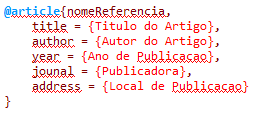
\includegraphics[scale=1]{./Imagens/capitulo_3/code_1.png}
	\end{center}
\end{figure}

Isso irá criar uma referencia, que poderá ser chamada em uma citação utilizando de 3 formas, citações diretas/indiretas curtas e longas, e  citações no texto.

Uma observação quanto a criação de referência, é que em muitas vezes o software não consegue reconhecer acentuações, então é preciso utilizar de comandos para inserir os acentos, os principais comandos são:
\begin{table}[htb]
	\IBGEtab{%
		\caption{Acentuação}%
		\label{tab_Cap3_acentos}
	}{%
		\begin{tabular}{cc}
			\toprule
			         Comando          & Acento \\ \midrule\midrule
			        \ba'\{a\}         &   á    \\
			       \ba ~\{a\}         &   ã    \\
			       \ba `\{a\}         &   à    \\
			\ba\textasciicircum \{a\} &   â    \\
			       \ba c\{c\}         &   ç    \\ \bottomrule
		\end{tabular}%
	}{%
		\fonte{Autoria Própria}%
	}
\end{table}
\subsection{Formas de Citações}
Uma citação direta ou indireta pode ser adicionado no próprio texto, conforme as normas citações com até três linhas, usando \lstinline|\citeonline{nomeReferencia}|. Por exemplo: ``Conforme dito por \citeonline{gajanan} tem-se que...''.

Outra forma de se fazer uma citação é de forma direta curta, como foi utilizado na tabela anterior, para fazer uma citação dessa forma, utiliza-se após a citação o comando \lstinline|\cite{nomeReferencia}|. Por exemplo: ``Existem centenas de estilos bibliográficos mundo a fora.''\cite{araujo2016}

Para citações grandes, com mais de 3 linhas, é preciso utilizar um ambiente especifico para citações longas \lstinline|\begin{citacao} Texto \cite{nomeReferencia}\end{citacao}|. Utilizando deste ambiente, é possível fazer citações da forma:
\begin{citacao}
	Três anos depois de ter anunciado uma descoberta há muito esperada pelos físicos, o bóson de Higgs, a Organização Europeia para a Pesquisa Nuclear (CERN, na sigla em francês) divulga a melhor representação da partícula já capturada até hoje. A imagem, apresentada nesta terça-feira (01/09/2015) durante uma conferência anual da instituição, foi o resultado da combinação dos dados coletados no Grande Colisor de Hádrons por dois experimentos diferentes, o ATLAS e o CMS, entre os anos de 2011 e 2012. \cite{oliveira2015}
\end{citacao}

Exite ainda uma 4º forma de realizar uma citação, mas neste caso, não existe citação em sí, apenas a inserção da referência na lista de bibliografia. Não recomendo utilizar está forma, mas caso seja necessário utilize o comando \lstinline|\nocite{nomeReferencia}|. Por exemplo, irei citar o livro Teorias de Aprendizagem de Marco Antônio Moreira sem apresentar nenhuma citação, apenas adicionando o comando \lstinline|\nocite{moreira2011}|. \nocite{moreira2011}

